


%%%%%%%%%%%%%%%%%%%%%%%%%%%%%%%%%%%%%%%%%%%%%%%%%%%%%%%%%%%%%%%%%%%%%%%%%%%%%%%
%%%%%%%%%%%%%%%%%%%%%%%%%%%%%%%%%%%%%%%%%%%%%%%%%%%%%%%%%%%%%%%%%%%%%%%%%%%%%%%
% APPENDIX
%%%%%%%%%%%%%%%%%%%%%%%%%%%%%%%%%%%%%%%%%%%%%%%%%%%%%%%%%%%%%%%%%%%%%%%%%%%%%%%
%%%%%%%%%%%%%%%%%%%%%%%%%%%%%%%%%%%%%%%%%%%%%%%%%%%%%%%%%%%%%%%%%%%%%%%%%%%%%%%

\section{Societal impact}
\label{appendix:societal_impact}
We believe that the paper has a positive societal impact for the following reasons:
\begin{itemize}
\item TS-LDDMM is an interpretable method for understanding inter-individual variability in biomedical datasets, potentially offering new insights in medicine.
\item TS-LDDMM bridges the gap between the shape analysis community and the unsupervised representation learning (URL) community, fostering potential future collaborations between these fields.
\end{itemize}
However, the computational cost of the method may raise environmental concerns similar to those associated with deep learning \cite{oh2024stable}.
 Additionally, while TS-LDDMM has promising biomedical applications, it could also be misused for creating poison.
\section{Proofs}
\label{appendix:proofs}
Denote by $\msg(s)\triangleq \{ (t,s(t)): \eqsp t\in \msi \} $ the graph of a time series $s: \msi \to \Rset^d$ and $ \phi.\msg(s)\triangleq\{ \phi(t,s(t)): \eqsp t\in \msi\} $ the action of  $\phi\in \mcd(\Rset^{d+1}) $ on $\msg(s)$.
\begin{theorem}
    \label{theorem:representation_proof}
Let $s:  \msj \to \Rset^d  $ and $\mathbf{s}_0: \msi\to \Rset^d $ be two continuously differentiable time seriess with $\msi,\msj$ two intervals of $\Rset$.
 There exist $f\in \rmC^1(\Rset^{d+1},\Rset^d)$ and $\gamma\in  \mcd(\Rset) $ such that $\gamma(\msi)=\msj $ and $\Phi_f\in \mcd(\Rset^{d+1})$,
 \begin{equation}% TO add more detail on functionnal space
    \msg(s)= \Pi_{\gamma,f}.\msg(\mathbf{s}_0),\eqsp \Pi_{\gamma,f}=\Psi_\gamma\circ\Phi_f.
 \end{equation}
 Moreover, for any $\bar{f}\in \rmC^1(\Rset^{d+1},\Rset^d)$ and $\bar{\gamma}\in  \mcd(\Rset) $, there exists a continously differentiable time series $\bar{s}$ such that 
 $\msg(\bar{s})= \Pi_{\bar{\gamma},\bar{f}}.\msg(\mathbf{s}_0)$
\end{theorem}
%\sam{preuve todo, classement des variétés à bord, donne un homeomorphisme sur la restriction}
\begin{proof}
  Let $s:  \msj \to \Rset^d  $ and $\mathbf{s}_0: \msi\to \Rset^d $ be two continuously differentiable time seriess with $\msi=(a,b),\msj=(\alpha,\beta)$ two intervals of $\Rset$.
  By setting $\gamma: t\in \Rset \mapsto (\beta-\alpha)(t-a)/(b-a)+\alpha\in \Rset $, we have $ \gamma(\msi)=\msj$ and $\gamma \in \mcd(\Rset) $.
   By defining $f:(t,x)\in\Rset^{d+1}\mapsto x-\mathbf{s}_0(t)+s\circ \gamma(t) $, the map $\Phi_f\in \mcd(\Rset^{d+1})$,
    indeed, its inverse is $\Phi_f^{-1}:(t,x)\in\Rset^{d+1}\mapsto (t,x+\mathbf{s}_0(t)-s(t)) $ and is continuously differentiable.
     Moreover, we have $\Pi_{\gamma,f}.\msg(\mathbf{s}_0)=\{(\gamma(t),s\circ \gamma(t)):\eqsp t\in\msi \}=\msg(s) $.

    

    Let $\bar{f}\in \rmC^0(\Rset^{d+1},\Rset^d)$, $\bar{\gamma}\in  \mcd(\Rset) $ and $\mathbf{s}_0\in \rmC^0(\msi,\Rset^d)$ with $\msi$ an interval of $\Rset$.
    We have :
    \begin{align}
      \Pi_{\gamma,f}.\msg(\mathbf{s}_0)&=\{(\gamma(t),f(t,\mathbf{s}_0(t))),\eqsp t\in \msi \} \\
      &\label{eq:proof1_last_eq}=\{(t,f\left(\gamma^{-1}(t),\mathbf{s}_0(\gamma^{-1}(t))\right),\eqsp t\in \gamma(\msi) \} \eqsp .
    \end{align}
    By defining $\bar{s}:t\in \gamma(\msi)\to f\left(\gamma^{-1}(t),\mathbf{s}_0(\gamma^{-1}(t))\right) $, we have $\bar{s}\in \rmC^0(\gamma(\msi), \Rset^d) $ by composition of continuous functions
    and $ \msg(\bar{s})= \Pi_{\gamma,f}.\msg(\mathbf{s}_0)$ by \eqref{eq:proof1_last_eq}, which concludes the proof.
\end{proof}
\begin{lemma}
  If we denote by $\msv$ the RKHS associated with the kernel $K_{\msg}$, then for any vector field $v$ generated by \eqref{eq:integration} with $v_0$ satisfying \eqref{eq:def_v0},
   there exist $\gamma \in \msd(\Rset) $ and $f\in \rmC^1(\Rset^{d+1},\Rset^d)$ such that $\phi^v=\Psi_\gamma\circ\Phi_f $.
\end{lemma}
\begin{proof}
  Let $v$ be a vector field generated by \eqref{eq:integration} with $v_0$ satisfying \eqref{eq:def_v0}.
 We remark that the first coordinate of the velocity field $v_\tau$ denoted by $v_\tau^{\text{time}}$ only depends on the time variable $t$ for any $\tau\in[0,1]$.
 Thus, when computing the first coordinate of the deformation $\phi^v$, denoted by $\gamma$, we integrate \eqref{eq:LDDMM_dynamic} with $v_\tau$ replaced by $v_\tau^{\text{time}}$,
  thus $\gamma$ is independant of the variable $x$. Moreover, $\gamma\in \mcd(\Rset)$ since a Gaussian kernel induced an Hilbert space $\msv$ satisfying $|f|_V\leq |f|_\infty+ |\dd f|_\infty  $ for any $f\in \msv$ by \citep[Theorem 9]{glaunes2005transport}.
  For the same reason, we have $\phi^v\in \mcd(\Rset^{d+1})$, and thus its last coordinates denoted by $f$ belongs to $\rmC^1(\Rset^{d+1},\Rset^d)$, and by construction $\phi^v=\Psi_\gamma\circ\Phi_f $.
\end{proof}




\section{Oriented varifold}

\label{appendix:varifold}
In this section, we introduce the \textit{oriented varifold} associated with curves.
For further readings on curves and surfaces representation as varifolds, readers can refer to \cite{kaltenmark2017general,charon2013varifold}. 
We associate to $\gamma\in \rmC^1((a,b),\Rset^{d+1})$ an \textit{oriented varifold} $\mu_\gamma$, i.e. a distribution on the space $\Rset^{d+1}\times \mathbb{S}^{d}$ defined as follows, for any smooth test function $\omega :\Rset^{d+1}\times \mathbb{S}^{d}\to \Rset  $,
\begin{equation}
  \mathbb{E}_{Y\sim \mu_\gamma}\left[\omega(Y)\right]=\mu_\gamma(\omega)=\int_a^b \omega\left(\gamma(t),\frac{\dot{\gamma}(t)}{|\dot{\gamma}(t)|}\right)|\dot{\gamma}(t)|\dd t \eqsp .
\end{equation}
Denoting by $\msw$ the space of smooth test function, we have that $\mu_\gamma $ belongs to its dual $\msw^*$.
 Thus, a distance on $\msw^*$ is sufficient to set a distance on oriented varifolds associated to curve and thus on $\rmC^1((a,b),\Rset^{d+1})$ by the identification $\gamma\to \mu_\gamma $.
Remark that in (TS-LDDMM), $\gamma$ should be the parametrization of a time series' graph $\msg(s)$, i.e. $\gamma: t\in \msi \to (t,s(t))\in\Rset^{d+1} $ denoting by $s:\msi \to \Rset^d$ the time series.
However, in practice, we work with discrete objects.
 That is why, we set $W$ as an RKHS to use its representation theorem.
 More specifically \citep[Proposition 2 \& 4]{kaltenmark2017general} encourages us to consider a kernel $k:(\Rset^{d+1} \times \mathbb{S}^d)^2\to \Rset$ such that there exist two positive and continuously differentiable kernels $k_{\pos}$ and $k_{\dir}$, 
 such that for any $(x,\overrightarrow{u}),(y,\overrightarrow{v}) \in (\Rset^{d+1} \times \mathbb{S}^d)^2$
 \begin{equation}
     k((x,\overrightarrow{u}),(y,\overrightarrow{v})) = k_{\pos}(x,y)k_{\dir}(\overrightarrow{u},\overrightarrow{v}) \eqsp,
   \end{equation}
 with moreover $k_\dir>0$ and $ k_\pos$ which admits an RKHS $\msw_\pos$ dense in the space of continous function on $\Rset^{d+1}$ vanishing at infinite \cite{carmeli2010vector}.

Given such a kernel $k:(\Rset^{d+1} \times \mathbb{S}^d)^2\to \Rset$
verifying \citep[Proposition 2 \& 4]{kaltenmark2017general}, we have that for any $(x,v)\in \Rset^{d+1}\times \mathbb{S}^{d}$, $\delta_{(x,\overrightarrow{v})}$ belongs to $\msw^*$ as a distribution and that the dual metric $\langle\cdot,\cdot \rangle_{\msw^*} $ satisfies for any $(x_1,v_1),(x_2,v_2)\in \left(\Rset^{d+1}\times \mathbb{S}^{d}\right)^2$,
\begin{equation}
  \langle\delta_{(x_1,\overrightarrow{v}_1)},\delta_{(x_2,\overrightarrow{v}_2)} \rangle_{\msw^*} =k((x_1,\overrightarrow{v}_1),(x_2,\overrightarrow{v}_2)) \eqsp .
\end{equation}
Thus, given two sets of triplets $X=(l_i,x_i,\overrightarrow{v}_i)_{i\in[T_0-1]}\in (\Rset\times \Rset^{d+1}\times \mathbb{S}^d)^{T_0-1},Y=(l_i',y_i,\overrightarrow{w}_i)_{i\in[T_1]}\in (\Rset\times \Rset^{d+1}\times \mathbb{S}^d)^{T_1-1}$ and denoting by 
\begin{equation}
  \label{eq:def_mu_X}
  \mu_X=\sum_{i=1}^{T_0} l_i \delta_{(x_i,\overrightarrow{v}_i)},\mu_Y=\sum_{i=1}^{T_1} l_i' \delta_{(y_i,\overrightarrow{w}_i)} \eqsp,
\end{equation}
 we have,
\begin{equation}
   |\mu_X-\mu_Y |_{\msw^*}^2 = \sum_{i,j = 1}^{T_0-1}l_i k((x_i,\overrightarrow{v_i}),(x_i,\overrightarrow{v_i}^0))l_j - 2 \sum_{i=1}^{T_0-1}\sum_{j=1}^{T_1-1}l_i k((x_i,\overrightarrow{v_i}),(y_i,\overrightarrow{w_i}))l_j' + \sum_{i,j = 1}^{T_1-1}l_i' k((y_i,\overrightarrow{w_i}),(y_i,\overrightarrow{w_i}))l_j' \eqsp.
\end{equation}
Then, using the identification $X\to \mu_X, Y\to \mu_Y$, we can define a distance on sets of triplets as $d_{\msw^*,3}(X,Y)=|\mu_X-\mu_Y|_{\msw^*}^2$.

Now, we aim to discretize the oriented varifold $\mu_\msg $ related to a time series' graph $\msg(s)$ by using a set of triplets.
This is carried out by using a discretized version of $\msg(s) $, i.e. $\tilde{\msg}=(g_i=(t_i,s(t_i)))_{i\in[T]}\in(\Rset^{d+1})^T$, in the following way: 
For any  $i\in[T-1]$, denoting the center and length of the $i^{th}$ segment $[g_i,g_{i+1}]$ by
$c_i = (g_i + g_{i+1})/2$, $l_i = \| g_{i+1}-g_{i}\|$, and the unit norm vector of direction $\overrightarrow{g_i g_{i+1}}$ by
 $\overrightarrow{v_i} = (g_{i+1}-g_{i})/l_i$, we define the set of triplets $X(\tilde{\msg})=(l_i,c_i,\overrightarrow{v_i})_{i\in[T-1]}$ and its related oriented varifold $\mu_{X(\tilde{\msg})}= \sum_{i=1}^{T-1}l_i \delta_{c_i,\overrightarrow{v_i}}$ as in \eqref{eq:def_mu_X}.
 This is a valid discretization of the oriented varifold $\mu_\msg$ according to \citep[Proposition 1]{kaltenmark2017general}: $\mu_{X(\tilde{\msg})}$ converges towards $\mu_\msg$ as the size of the descretization mesh $\sup_{i\in[T-1]} |t_{i+1}-t_i| $ converges to 0.

 Finally, we define a distance on discretized time series' graphs $\tilde{\msg}_1,\tilde{\msg}_2$ as $d_{\msw^*}(\tilde{\msg}_1,\tilde{\msg}_2)=d_{\msw^*,3}(X(\tilde{\msg}_1),X(\tilde{\msg}_2)) $.


\subsection{Varifold kernels}
\label{appendix:kernel_implementation}
Denote the one-dimensional Gaussian kernel by $K_\sigma^{(a)}(x,y)=\exp(-|x-y|^2/\sigma)$ for any $(x,y)\in (\Rset^a)^2$, $a\in \Nset$ and $\sigma>0$.
In the implementation, we use the following kernels, for any $((t_1,x_1),(t_2,x_2))\in (\Rset^{d+1})^2, ((w_1,v_1),(w_2,v_2))\in (\mathbb{S}^{d})^2 $,
\begin{equation}
  k_{\pos}(x,y)=K_{\sigma_{\pos,t}}^{(1)}(t_1,t_2)K_{\sigma_{\pos,x}}^{(d)}(x_1,x_2),\quad k_{\pos}(x,y)=K_{\sigma_{\dir,t}}^{(1)}(w_1,w_2)K_{\sigma_{\dir,x}}^{(d)}(v_1,v_2)\eqsp ,
\end{equation}
where $\sigma_{\pos,t}, \sigma_{\pos,x}, \sigma_{\dir,t}, \sigma_{\dir,x}>0 $ are hyperparameters.
 In practice, we select $\sigma_{\pos,x}\approx \sigma_{\dir,x} \approx 1$ when the times series are centered and normalized. Otherwise we select $\sigma_{\pos,x}\approx \sigma_{\dir,x} \approx \bar{\sigma}_{s}$ with $\bar{\sigma}_{s}$ the average standard deviation of the time series.
  We choose $\sigma_{\pos,t}\approx \sigma_{\dir,t} = m f_e$ with $f_e$ the sampling frequency of the time series and $m\in [5]$ an integer depending on the time change between the starting and the target time series graph.
  The more significant the time change, the higher $m$ should be. The intuition comes from the fact that the width $\sigma_{\pos,t}, \sigma_{\dir,t}$ rules the time windows used to perform the comparison, and $\sigma_{\pos,x}, \sigma_{\dir,x}$ affects the space window.
   The size of the windows should be selected depending on the variations in the data.

\section{Tuning the hyperparameters of the TS-LDDMM velocity field kernel}
\label{appendix:kernel_TS_LDDMM}
The parameter $\sigma_{T,0}$ should be chosen \textit{large} compared the sampling frequency $f_e$ and compared to average standard deviation $\bar{\sigma}_s$ of the time series, e.g $\sigma_{T,0}=100$ as $\bar{\sigma}_s\approx f_e\approx  1 $.
It makes the time transformation smoother. If $\sigma_{T,0}$ is too small, for instance, $\sigma_{T,0}=f_e $, the effect of the time deformation is too localized, and there are not enough samples to make it visible.

The parameter $\sigma_{T,1}$ should be of the same order as $f_e$: two different points in time can have various space transformations.
 $\sigma_x$ should be of the same order of $\bar{\sigma}_s$: two points with a big difference regarding space compared to $\bar{\sigma}_s$ can have very different space transformations.

 We take $c_0\approx 10 c_1 $, we want to encourage time transformation before space transformation. We take $(c_0,c_1)=(1,0.1)$ in all experiments.


\section{Experimental settings}
\label{appendix:settings}
All experiments were performed on a Debian 6.1.69-1 server with NVIDIA RTX A2000 12GB GPU, Intel(R) Xeon(R) Gold 5220R CPU @ 2.20GHz, and 250 GB of RAM. The source code will be available on Github.

\subsection{Optimization details of TS-LDDMM \& LDDMM}
\label{appendix:optimizers_details}

We implemented TS-LDDMM in Python with the JAX library \footnote{https://github.com/google/jax}.

\paragraph{Initialization.}
As initialization of \eqref{eq:general_optimization_problem}, all momentum parameters are set to $0$, and the initial graph of reference is picked from the dataset such that its length is equal to the median length observed in the dataset.

\paragraph{Gradient descent.}
The chosen gradient descent method is "adabelief" \cite{zhuang2020adabelief} implemented in the OPTAX library~\footnote{https://optax.readthedocs.io/en/latest/}.
The gradient descent has two main parameters: the number of steps (nb\_steps) and the maximum stepsize value ($\eta_M$).
The stepsize has a scheduling scheme: 
\begin{itemize}
  \item Warmup period on $0.1 \times$ nb\_steps steps: the stepsize increases linearly from $0$ to $\eta_M$. The goal is to learn progressively the parameters. If the step size is too large at the start, smaller steps at the end cannot make up for the mistakes made at the beginning. 
  \item Fine tuning periode on $ 0.9  \times$ nb\_steps : the stepsize decreases from $\eta_M$ to $0$ with a cosine decay implemented in the OPTAX scheduler, i.e. the decreasing factor as the form $0.5  (1 + \cos(\pi  t/T))$. 
\end{itemize}
By default, we set nb\_steps to 400 and $\eta_M$ to 0.1.

\section{Datasets}
\subsection{Mouse respiratory cycle dataset}

\begin{figure}
  \centering
  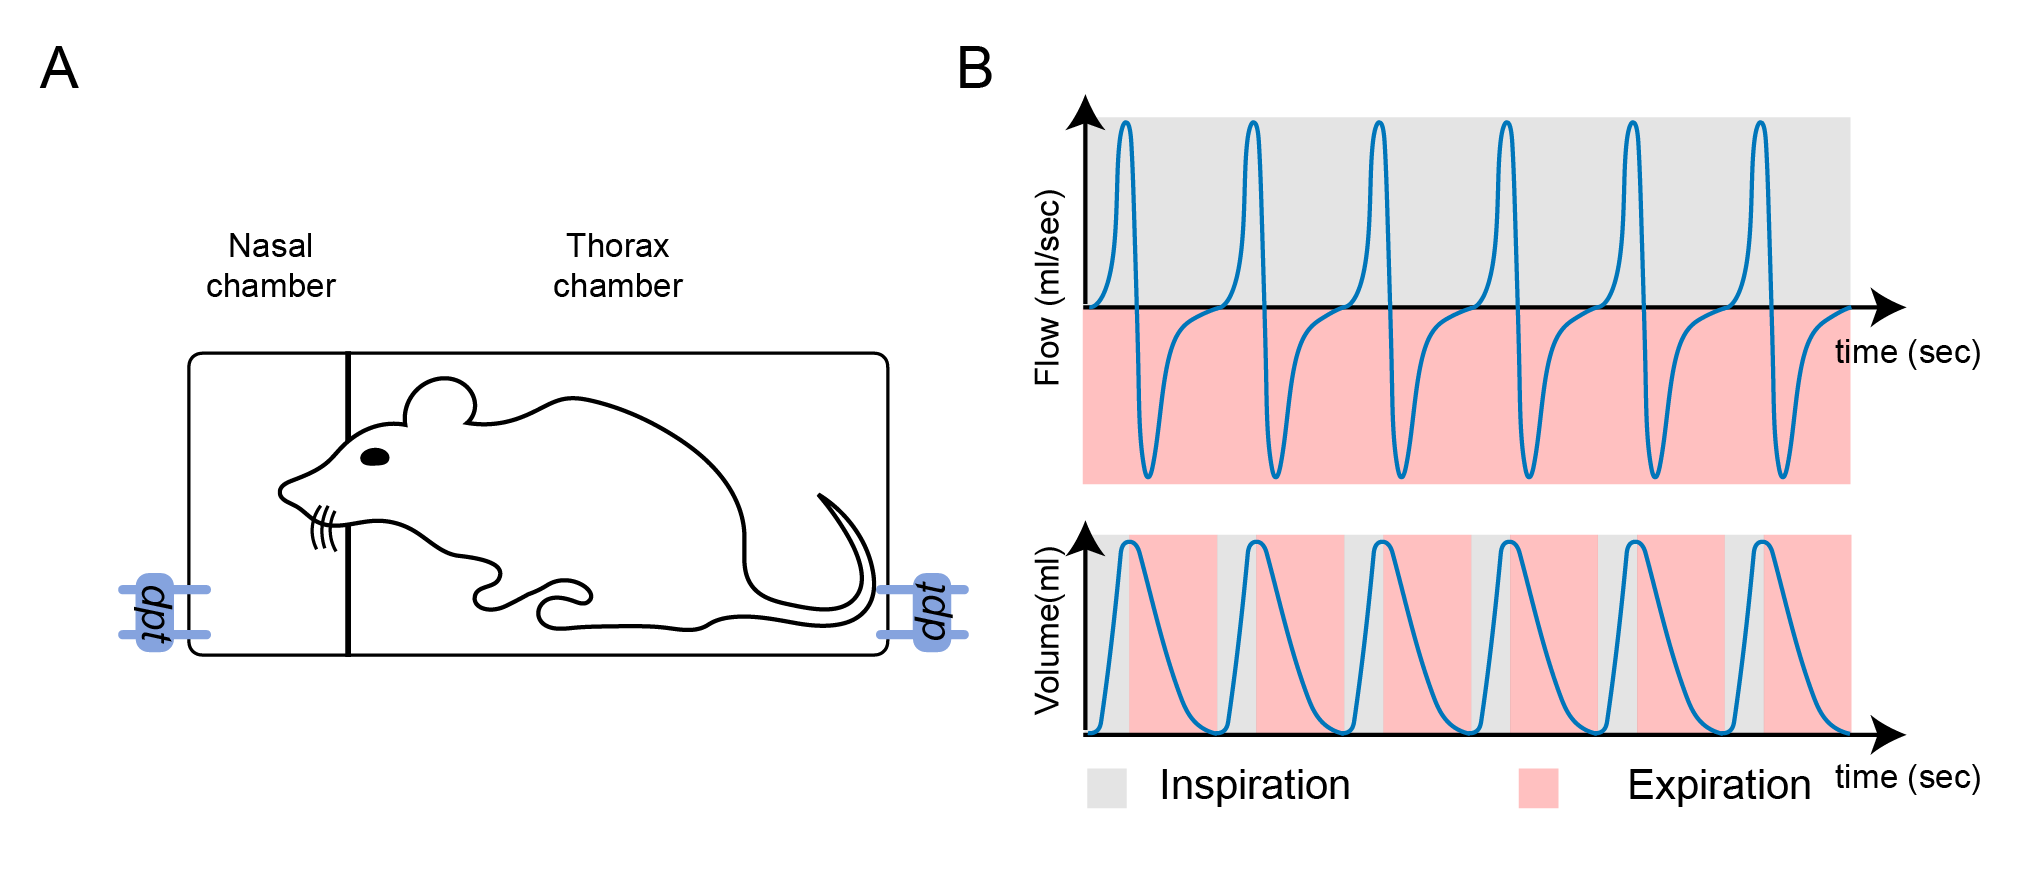
\includegraphics[width = \linewidth]{pictures/mice_exp.png}
  \caption{A: Illustration of a double-chamber plethysmograph. The term \textit{dpt} stands for differential 
  pressure transducer which measures the pressure in each compartment, the pressure then being converted to flow. 
  B: Nasal airflow (top) and lung volume (bottom). During inspiration, airflow is positive (grey) and during
  expiration, airflow is negative (pink).}
  \label{fig:mice_exp}
\end{figure}

\label{appendix:mouse_dataset}
Ventilation is a simple physiological function that ensures a vital supply of oxygen and the elimination of CO2. 
Acetylcholine (Ach) is a neurotransmitter that plays an important role in muscular activity, notably for breathing. 
Indeed, muscle contraction information passes from the brain to the muscle through the nervous system. Achs are located 
in synapses of the nervous system (central and peripheral) and skeletal muscles. They ensure the information transmission 
from nerve to nerve. However, the transmission cannot end without the hydrolysis of Ach by the enzyme Acetylcholinesterase 
(AchE), allowing nerves to return to their resting state. Inhibition of (AchE) with, for instance, nerve gas, pesticide, 
or drug intoxication leads to respiratory arrests. 

The dataset comes from the experiment \cite{nervo2019respiratory}, where they studied the consequences of partial 
deficits in AChE and AChE inhibition on mice respiration. AchE inhibition was induced with an 
irritant molecule called physostigmine (an AchE inhibitor). Mice nasal airflows were sampled at 
2000Hz with a Double Chamber plethysmograph \cite{hoymann2012lung}, as depicted in \Cref{fig:mice_exp}-A). The flow is expressed in 
$ml.s^{-1}$; it has a positive value during inspiration and a negative value expiration \Cref{fig:mice_exp}-B). 
Among the mice population, we selected 7 control mice (\textbf{wt}) and 7 ColQ mice (\textbf{colq}), which do not have 
AChE anchoring in muscles and some tissues. 
As described in \cite{nervo2019respiratory}, mice experiments were as follows:
\begin{enumerate}
  \item The mouse is placed in a DCP for 15 or 20 min to serve as an internal control.
  \item The mouse is removed from the DCP and injected with physostigmine.
  \item The mouse is placed back into the DCP, and its nasal flow is recorded for 35 or 40 min.
\end{enumerate}

Respiratory cycles were extracted following procedure \cite{germain2023unsupervised}. We removed 
respiratory cycles whose duration exceeds 1 second; the average respiratory cycle duration is 
300 ms. We randomly sampled 10 respiratory cycles per minute and mouse. It leads to a dataset of 
12,732 (time, genotype)-annotated respiratory cycles. 

\subsection{Shape-based UCR/UEA time series classification datasets}
\label{appendix:classification_dataset}
We selected 15 shape-based datasets (7 univariates and 8 multivariates) from the from the University of East Anglia (UEA) and the University of California Riverside (UCR) Time Series Classification Repository\footnote{https://timeseriesclassification.com} \cite{dau2019ucr,bagnall2018uea}. All datasets were downloaded with the python package aeon\footnote{https://www.aeon-toolkit.org/en/stable/}. Essential datasets information are summarized in \Cref{appendix:table:datasets} and further can be found in \cite{dau2019ucr,bagnall2018uea}.

\begin{table}[hbt!]
  \centering
  \caption{UCR/UEA shape-based time series datasets for classification.}
  \resizebox{\columnwidth}{!}{%
  \begin{tabular}{lllllll}
    \toprule
    & \textbf{Dataset} &  \textbf{Size} & \textbf{Lengh} & \textbf{Number of classes} & \textbf{Number of dimensions} & \textbf{Type} \\
    \midrule
    \multirow[c]{7}{*}{Univariate} &  ArrowHead & 211 & 251 & 3 & 1 & IMAGE \\
    & BME & 180 & 128 & 3 & 1 & SIMULATED \\
    & ECG200 & 200 & 96 & 2 & 1 & ECG \\
    & FacesUCR & 2250 & 131 & 14 & 1 & IMAGE \\
    & GunPoint & 200 & 150 & 2 & 1 & MOTION \\
    & PhalangesOutlinesCorrect & 2658 & 80 & 2 & 1 & IMAGE \\
    & Trace & 200 & 275 & 4 & 1 & SENSOR \\
    \cline{1-7}
    \multirow[c]{8}{*}{Multivariate}& ArticularyWordRecognition & 575 & 144 & 25 & 9 & SENSOR \\
    & Cricket & 180 & 1197 & 12 & 6 & MOTION \\
    & ERing & 60 & 65 & 6 & 4 & SENSOR \\
    & Handwriting & 1000 & 152 & 26 & 3 & MOTION \\
    & Libras & 360 & 45 & 15 & 2 & VIDEO \\ 
    & NATOPS & 360 & 51 & 6 & 24 & MOTION \\
    & RacketSports & 303 & 30 & 4 & 6 & SENSOR \\
    & UWaveGestureLibrary & 240 & 315 & 8 &3 & SENSOR \\
    \bottomrule
  \end{tabular}
  %
  }
  \label{appendix:table:datasets}
\end{table}

\section{Appendix for experiment: TS-LDDMM representation identifiability}
\label{appendix: identifiability}
In this experiment, we evaluate the ability of TS-LDDMM to retrieve the parameter $v_0^*$ that encodes the deformation $\varphi^{\{v_0^*\}}$ acting on a time series graph $\msg$ by solving the geodesic shooting problem \eqref{eq:relaxation} between $\msg$ and $\varphi^{\{v_0^*\}}.\msg$. Parameter identifiability is an important property for subsequent statistical analysis. Results show that TS-LDDMM representations are identifiable or weakly identifiable depending on the velocity field kernel $K_G$ specification.

\subsection{Settings}
\label{appendix: settings_identifiability}
This experiment only involves the TS-LDDMM method in two different settings: 
\begin{itemize}
  \item \textbf{The velocity field kernel $K_G$ is well-specified:} The velocity field kernel $K_G$ is set to $ (c_0,c_1,\sigma_{T,0},\sigma_{T,1},\sigma_x) = (1,0.1,100,1,1)$, the varifold loss kernels $(k_{pos},k_{dir})$ are set to $(\sigma_{\pos,t}, \sigma_{\pos,t}, \sigma_{\dir,t}, \sigma_{\dir,x}) = (2,1,2,0.6)$, and the optimizer has 400 steps with a maximum stepsize $\eta_M$ of 0.05.
  \item \textbf{The velocity field kernel $K_G$ is missspecified:} The velocity field kernel $K_G$ is set with  $(c_0,c_1,\sigma_{T,1}) = (1,0.1,1)$, $\sigma_{T,0}$ ranging in $(1,5,10,50,100,200,300)$, and $\sigma_x$  ranging in $(0.1,1,10,100)$. The varifold loss kernels $(k_{pos},k_{dir})$ are set to $(\sigma_{\pos,t}, \sigma_{\pos,t}, \sigma_{\dir,t}, \sigma_{\dir,x}) = (2,1,2,0.6)$, and the optimizer has 400 steps with a maximum stepsize $\eta_M$ of 0.05.
\end{itemize}

\begin{figure}[t]
  \centering
  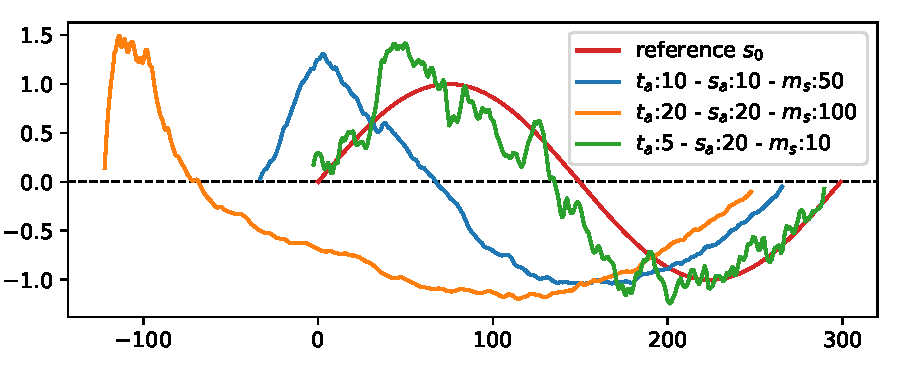
\includegraphics[width=0.5\linewidth]{pictures/samples.pdf}
  \caption{Plots of $\varphi^{\{v_0(\mathbf{\alpha}^*,\msx)\}}.\msx$ for different values of $\mathbf{\alpha}^*$ according to its sampling parameter $t_a,s_a,m_s $, taking $\msx=\msg(s_0)$ with $s_0:k\in [300]\to \sin(2\pi k/300) $.}
  \label{fig:exemple_synthetic}
\end{figure}

\begin{table}
  \caption{Values of $\scrl(\varphi^{\{v_0(\mathbf{\alpha}^*,\msx)\}}.\msx,\varphi^{\{\hat{v}_0\}}.\msx)$ as $\mathbf{\alpha}^*$ is sampled according to Gen(10,10,50) and $\hat{v}_0$ is estimated using $K_\msg$ with varying parameters $\sigma_{T,1},\sigma_x$.}
    \centering
       \begin{tabular}{lrrrrrrr}
       \toprule
       $\sigma_{T,0} \backslash \sigma_x$  & 1 & 10 & 50 & 100 & 200 & 300 \\
       \midrule
       0.1 & 2e+0 & 3e-4  & 1e-5&4e-6&7e-4&4e-3 \\
      1 & 4e-2 & 1e-4  & 1e-5&4e-6&7e-4 &4e-3  \\
       100 & 4e-2 & 2e-4  & 1e-5&4e-6&7e-4&4e-3  \\
       \bottomrule
       \end{tabular}
    \label{table:synthetic2}
\end{table}

provided that the hyperparameters and the reference graph are wisely selected, i.e., the parameter $v_0^*$ generating a deformation $\varphi^{\{v_0^*\}}$ of a time series graph $\msg$ can be estimated from the data $\msg,\varphi^{\{v_0^*\}}.\msg$ by solving the geodesic shooting problem \eqref{eq:relaxation}. 

\paragraph{The velocity field kernel $K_G$ is well specified.}

First, we show the model identifiability when the kernel $K_G$ is well specified: the estimated parameter is a good approximation of the generating parameter when the generation and the estimation procedure use the same hyperparameters for the RKHS kernel $K_\msg$.
All the hyperparameter values for generation and estimation are given in \Cref{appendix: settings_identifiability}.

We fix the initial control points as $\msx=\left(x_k=(k,\sin(2\pi k/300))\right)_{k\in[300]} $.
Given $m_{s}\in \Nset_{>0}$ and $t_{a},s_{a}>0$, we randomly generate initial momentums $\mathbf{\alpha}^*=(\alpha_k^*)_{k\in[\mathbf{n}_0]}$ with the following sampling, called Gen($m_s,t_a,s_a$):
For any $k\in[\mathbf{n}_0]$, $\mathbf{\alpha}_k'$ is sampled according to a Gaussian normal distribution $\mathcal{N}(0_{d+1},I_{d+1})$.
Then, $(\alpha_k')_{k\in[\mathbf{n}_0]}$ is regularized by a rolling average of size $m_{s}$, we get $\bar{\mathbf{\alpha}}'=(\bar{\alpha}_k')_{k\in[\mathbf{n}_0]}$.
Finally, we normalize $\bar{\mathbf{\alpha}}'$ to derive $\mathbf{\alpha}^*$ such that $|([\alpha_k^*]_t)_{k\in[\mathbf{n}_0]}|=t_{\text{amp}}$ and $|([\alpha_k^*]_s)_{k\in[\mathbf{n}_0]}|=s_{\text{amp}}$ for any $k\in[\mathbf{n}_0]$, denoting by $[\alpha_k^*]_t,[\alpha_k^*]_s$ the time and space coordinates of $\alpha_k^*$ respectively.
Note that the regularizing step $(\mathbf{\alpha}_k')_{k\in[\mathbf{n}_0]}\to \bar{\mathbf{\alpha}}' $ is necessary to obtain realistic deformations which take into account the regularity induced by the RKHS $\msv$.

Then, using $v_0(\mathbf{\alpha}^*,\msx)$ as defined in \eqref{eq:def_v0} with initial momentums $\mathbf{\alpha}^*$ and control points $\msx$, we apply the induced deformation $\varphi^{\{v_0\}} $ by \eqref{eq:integration} to $\msx$ and obtain $\varphi^{\{v_0\}}.\msx$.
Finally, we solve \eqref{eq:relaxation} to recover an estimation $\hat{\mathbf{\alpha}}$ of $\mathbf{\alpha}^*$ and report the average relative error (ARE) $|v_0(\hat{\mathbf{\alpha}},\msx)-v_0(\mathbf{\alpha}^*,\msx)|_\msv/|v_0(\mathbf{\alpha}^*,\msx)|_\msv$ on 50 repetitions.
This procedure is performed for any $m_{s},t_{a},s_{a}\in \{10,50,100\}\times \{5,10,15,20\}^2 $.
Mean, standard deviation, and maximum of the ARE on all these hyperparameters choices are respectively $\mathbf{0.10, 0.03, 0.17}$.
Therefore, the estimation procedure \eqref{eq:relaxation} offers a good approximation of the true parameter when the kernel $K_\msg$ is well specified.
We observe that the estimation is difficult when $t_a\ll s_a$ because the time series can be very noisy as illustrated in \Cref{fig:exemple_synthetic}: this impacts the Varifold loss which is sensitive to tangents.

\paragraph{The velocity field kernel $K_G$ is misspecified.}

We demonstrate a weak identifiability when the kernel $K_\msg$ is misspecified: we can reconstruct the graph time series' after deformations even if the hyperparameters of $K_\msg$
are different during the generation and the estimation.
 The hyperparameters of $K_\msg$ during generation are $(c_0,c_1,\sigma_{T,0},\sigma_{T,1},\sigma_x)=(1,0.1,100,1,1)$ and we fix $\sigma_{T,1},c_0,c_1=(1,1,0.1) $ for $K_\msg$ during estimation.
 We aim to understand the impact of $\sigma_{T,1},\sigma_x$ on the reconstruction since they are encoding the smoothness of the transformation according to time and space.  

For any choice of the hyperparameters $\sigma_{T,1},\sigma_x\in \{1,10,50,100,200,300 \}\times \{0.1,1,100\}$ related to $K_\msg$ in the estimation,
we average $\scrl(\varphi^{\{v_0(\mathbf{\alpha}^*,\msx)\}}.\msx,\varphi^{\{\hat{v}_0\}}.\msx)$ on 50 repetitions when $\mathbf{\alpha}^*$ is sampled according to Gen$(10,10,50)$ and $\hat{v}_0=v_0(\hat{\alpha},\msx)$ denoting by $\hat{\alpha}$ the result of the minimization \eqref{eq:relaxation}.
We observe in \Cref{table:synthetic2} that the reconstruction is almost perfect except in the case when $\sigma_{t,0}=1$ during estimation, while $ \sigma_{t,0}=100$ during generation.
Compared to $\sigma_{T,0}$, $\sigma_x$ has nearly no impact on the reconstruction.
In \Cref{appendix:kernel_implementation}-\ref{appendix:kernel_TS_LDDMM}, we propose guidelines to drive future hyperparameters tuning and further discussions related to $\sigma_{T,1},c_0,c_1$. 

\section{Appendix for experiment: Robustness to irregular sampling}
\label{appendix: robustness}

This experiment is inspired by \cite{oh2024stable} where the authors perform an extensive comparison of Neural Ordinary Differential Equations (Neural ODEs) methods~\cite{kidger2020neural}. We assess the classification
performances of several methods under regular sampling (0\% missing rate) and three irregular sampling regimes on 15 shape-based datasets (7 univariate \& 8 multivariate). Methods and training strategy are taken from its associated Github\footnote{\url{https://github.com/yongkyung-oh/Stable-Neural-SDEs}} and described in what follows. We conclude with the results, which show that our method, TS-LDDMM, outperforms all methods for sampling regimes with missing rates: 0\%, 30\%, and 50\%.

\subsection{Benchmark methods}
\label{appendix: benchmark robustness}
In related work, we give an overview of Neurals ODEs methods and their relation with TS-LDDMM.  
\begin{itemize}
  \item RNN-based methods: Baseline reccurent neural networks including RNN~\cite{medsker1999recurrent}, LSTM~\cite{hochreiter1997long}, and GRU~\cite{chung2014empirical}.

  \item Attention-based methods: Multi-Time Attention Networks (MTAN)~\cite{shukla2021multi} and Multi-Integration Attention Module (MIAM)~\cite{lee2022multi}. Both handle multivariate time series irregularly sampled with attention mechanisms.
  \item Neural ODEs: ODE-LSTM~\cite{lechner2020learning} a form of Neural-ODEs used to learn continuous latent representations. 
  \item Neural SDEs:  Neural SDE~\cite{liu2019neural} and Neural LNSDE~\cite{oh2024stable} have been proposed to model randomness in time-series using drift and diffusion terms as an extension of Neural-ODEs. 
  \item Shape-Analysis methods: TS-LDDMM (ours) and LDDMM~\cite{glaunes2008large}. From shape analysis, both methods learn representations by solving ODEs parametrized with Kernels. While both methods handle multivariate signals irregularly sampled, TS-LDDMM is specifically designed for time series.
\end{itemize}

\subsection{Model architecture}

\paragraph{Neural ODEs methods}
As depicted in~\cite{oh2024stable}, any Neural ODEs layer in \Cref{appendix: benchmark robustness} is followed by an MLP with two fully connected layers with \texttt{ReLU} activations. The risk of overfitting and the model regularization are handled with a dropout rate of 10\% and an early-stopping mechanism, ceasing the training when the validation loss does not improve for 10 successive epochs. 

For each method and dataset, the learning rate, the hidden vector dimensions, and the number of layers are optimized to minimize the CrossEntropy loss on a validation set using the \texttt{Ray}~\footnote{\url{https://github.com/ray- project/ray}} Python library. 
The learning rate varies from $10^{-4}$ to $10^{-1}$ using log uniform search, the hidden vector dimension ranges from ${16, 32, 64, 128}$ using grid search, and the number of layers ranges from ${1, 2, 3, 4}$ using grid search. The batch size was selected from ${16, 32, 64, 128}$ according to the size of the dataset. All methods were trained for 100 epochs, and the best method was selected based on the lowest validation loss. 

\paragraph{TS-LDDMM and LDDMM}
Representations learned with TS-LDDMM or LDDMM are fed to a Support Vector Classifier (\href{https://scikit-learn.org/stable/modules/generated/sklearn.svm.SVC.html#sklearn.svm.SVC}{SVC}) from \texttt{scikit-learn}~\footnote{\url{https://scikit-learn.org/stable/}}. All SVC's hyperparameters are set to default except the regularization term C, which is set through grid search on a validation set with the macro f1-score~\footnote{\url{https://scikit-learn.org/stable/modules/generated/sklearn.metrics.f1_score.html}}. 

To learn TS-LDDMM (resp. LDDMM) representations, the velocity field kernel $K_G$ is set to $ (c_0,c_1,\sigma_{T,0},\sigma_{T,1},\sigma_x) = (1,0.1,0.33\bar{l},1,n_d)$, (resp. $ (\sigma_{T},\sigma_x) = (0.33\bar{l},n_d)$) where $\bar{l}$ is the average time series length and $n_d$ the number of dimensions. For both methods and all datasets, the varifold loss kernels $(k_{pos},k_{dir})$ are identical and set to $(\sigma_{\pos,t}, \sigma_{\pos,t}, \sigma_{\dir,t}, \sigma_{\dir,x}) = (2,n_d,2,n_d)$. For TS-LDDMM (resp. LDDMM), the optimizer is set with 400 epochs (resp. 400) and a maximum learning rate $\eta_M = 0.1$ (resp. $\eta_M = 0.01$). In all cases, the initial reference graph is selected in the dataset as a time series with the median length.


\subsection{Protocol}

In this experiment, we investigate the robustness to missing samples and the classification performance of TS-LDDMM compared to Neural ODEs on 15 datasets described in \Cref{appendix:classification_dataset}. For fairness between methods of different architectures, the evaluation protocol on each dataset and method is as follows: 
\begin{enumerate}
  \item Spilt the dataset in train 75\%, validation 15\%, and test 15\%.
  \item Tune hyperparameters with train and validation sets and a missing rate of 0\%.
  \item For each missing rate in [0\%,30\%,50\%,70\%]
    \begin{itemize}
      \item Remove samples in time series in the train and test sets according to the missing rate and the drop procedure described in~\cite{kidger2020neural}.
      \item Train the model on the train set
      \item Evaluate the macro f1-score on the test set
    \end{itemize}
\end{enumerate}




\subsection{Results}
In this experiment, we investigate the robstuness to missing samples and the classification performance of TS-LDDMM representations. We compare TS-LDDMM with LDDMM and 8 neural ODEs networks. Performances are evaluated in terms of average macro f1-score and rank on four different regimes of missing rate 0\%,30\%,50\%, and 70\%. Results are aggregated in \Cref{table:robstuness}. 

On three out of four regimes (0\%,30\%, and 50\%) TS-LDDMM classifier is the best performer in terms of f1-score and rank. For missing rates of 0\% and 30\%, the score increases by 10\% compared to the second-best performer, LDDMM. However, LDDMM is not the second-best performer in rank (Neural LNSDE), showing its sensitivity to parameterization, unlike TS-LDDMM, which remains consistent. Performances of Neural LNSDE remain constant with the increase of the missing rate as observed in~\cite{oh2024stable}, and it becomes the best performer for missing rate 70\%. The decrease in TS-LDDMM performances with the increasing missing rate is due to the varifold loss, which poorly approximates the time series shape. Other losses might be more relevant for high missing rates.

Overall, TS-LDDMM is a relevant and consistent shape-based representation for irregularly sampled multivariate time series for missing rates up to 50\% . 

\begin{table}[hbt!]
  \centering
  \caption{Comparison of average macro f1-score and rank as the sample dropping rate increases. \textbf{First} \& \underline{second} best performers. TS-LDDMM is the best performer on three out of four regimes.}
  \label{table:robstuness}
  \resizebox{\columnwidth}{!}{%
  \begin{tabular}{lcccccccc}
    \toprule
    \multirow[c]{2}{*}{\textbf{Methods}} & \multicolumn{2}{c}{\textbf{Regular}} & \multicolumn{2}{c}{\textbf{30 \% dropped}} &  \multicolumn{2}{c}{\textbf{50 \% dropped}} & \multicolumn{2}{c}{\textbf{70 \% dropped}} \\
    \cline{2-9}
     &  \textbf{F1-score} & \textbf{Rank} &  \textbf{F1-score} & \textbf{Rank} &  \textbf{F1-score} & \textbf{Rank} &  \textbf{F1-score} & \textbf{Rank} \\
    \midrule
    RNN (1999) & $0.64 \pm 0.21$  & 6.2 & $0.53 \pm 0.23$  & 6.6 & $0.48 \pm 0.21$  & 7.2 & $0.44 \pm 0.21$  & 6.07 \\
    LSTM (1997) & $0.61 \pm 0.29$  & 6.0 & $0.57 \pm 0.29$  & 6.27 & $0.53 \pm 0.25$  & 6.07 & $0.51 \pm 0.29$  & 5.27 \\
    GRU (2014) & $0.71 \pm 0.26$  & 4.2 & $0.68 \pm 0.28$  & 4.27 & $0.66 \pm 0.28$  & 3.73 & $\underline{0.59 \pm 0.28}$  & \underline{3.67} \\
    MTAN (2021) & $0.59 \pm 0.28$  & 7.13 & $0.58 \pm 0.28$  & 5.8 & $0.54 \pm 0.29$  & 5.33 & $0.51 \pm 0.28$  & 5.0 \\
    MIAM (2022) & $0.48 \pm 0.35$  & 6.93 & $0.42 \pm 0.33$  & 8.27 & $0.47 \pm 0.31$  & 6.93 & $0.35 \pm 0.31$  & 7.6 \\
    ODE-LSTM (2020) & $0.63 \pm 0.24$  & 6.0 & $0.57 \pm 0.25$  & 6.53 & $0.51 \pm 0.24$  & 7.27 & $0.45 \pm 0.23$  & 6.73 \\
    Neural SDE (2019) & $0.48 \pm 0.28$  & 7.67 & $0.47 \pm 0.26$  & 7.47 & $0.45 \pm 0.27$  & 7.13 & $0.45 \pm 0.25$  & 6.0 \\
    Neural LNSDE (2024) & $0.7 \pm 0.27$  & \underline{3.87} & $0.68 \pm 0.29$  & \underline{4.0} & $\underline{0.67 \pm 0.25}$  & \underline{3.53} & $\mathbf{0.66 \pm 0.23}$  & \textbf{2.47} \\
    LDDMM (2008) & $\underline{0.72 \pm 0.2}$  & 4.53 & $\underline{0.7 \pm 0.21}$  & 4.2 & $0.57 \pm 0.25$  & 5.0 & $0.4 \pm 0.25$  & 7.13 \\
    TS-LDDMM (ours) & $\mathbf{0.83 \pm 0.18}$  & \textbf{2.93} & $\mathbf{0.8 \pm 0.18}$  & \textbf{2.07} & $\mathbf{0.7 \pm 0.26}$  & \textbf{3.33} & $0.51 \pm 0.27$  & 5.67 \\
    \bottomrule
  \end{tabular}  
  %
  }
\end{table}







\section{Appendix for experiment: Classification benchmark on regularly sampled datasets}
\label{appendix: shape_classification}

In this section, we compare the classification performances of TS-LDDMM with other methods from shape analysis on 15 shape-based datasets of time series regularly sampled. TS-LDDMM outperforms other methods on 12 out of 15, highlighting its relevance for shape analysis when dealing with time series. 


\subsection{Benchmark metohds}
\begin{itemize}
  \item SRV-based method: we include TCLR~\cite{heo2024logistic} a logistic regression on the tangent space of the Frechet mean with Square Root Velocity (SRV representation). We also include Shape-FPCA~\cite{wu2024shape} that encodes both the time series and its time parameterization. 
  \item LDDMM-Based : TS-LDDMM (ours) and LDDMM~\cite{glaunes2008large}. Both methods learn representations by solving ODEs parametrized with Kernels. While both methods handle multivariate signals, TS-LDDMM is specifically designed for time series.
 \end{itemize}

\subsection{Model settings}

\paragraph{TCLR \& Shape-FPCA}
Shape-FPCA is available in the Python library \texttt{FDASRSF}~\footnote{https://fdasrsf-python.readthedocs.io/en/latest/}. Once the shape-FPCA representations are learned, they are fed to an \href{https://scikit-learn.org/stable/modules/generated/sklearn.svm.SVC.html#sklearn.svm.SVC}{SVC} from \texttt{scikit-learn}. \texttt{FDASRSF} provides SRV representation methods that we combined with a \href{https://scikit-learn.org/stable/modules/generated/sklearn.linear_model.LogisticRegressionCV.html}{logistic regression} from \texttt{scikit-learn} to implement TCLR. For both methods, the number of steps to learn the Frechet mean is set to 50, and the regularization hyperparameter C is set through grid search on a validation set with the macro f1-score. Other parameters are set to default.  

\paragraph{TS-LDDMM \& LDDMM}
Representations learned with TS-LDDMM or LDDMM are fed to an SVC from \texttt{scikit-learn}. All SVC's hyperparameters are set to default except the regularization term C, which is set through grid search on a validation set with the macro f1-score. 

To learn TS-LDDMM (resp. LDDMM) representations, the velocity field kernel $K_G$ is set to $ (c_0,c_1,\sigma_{T,0},\sigma_{T,1},\sigma_x) = (1,0.1,0.33\bar{l},1,n_d)$, (resp. $ (\sigma_{T},\sigma_x) = (0.33\bar{l},n_d)$) where $\bar{l}$ is the average time series length and $n_d$ the number of dimensions. For both methods and all datasets, the varifold loss kernels $(k_{pos},k_{dir})$ are identical and set to $(\sigma_{\pos,t}, \sigma_{\pos,t}, \sigma_{\dir,t}, \sigma_{\dir,x}) = (2,n_d,2,n_d)$. For TS-LDDMM (resp. LDDMM), the optimizer is set with 400 epochs (resp. 400) and a maximum learning rate $\eta_M = 0.1$ (resp. $\eta_M = 0.01$). In all cases, the initial reference graph is selected in the dataset as a time series with the median length.


\paragraph{Protocole}
For each dataset and method, the evaluation protocol is a simple train,validation test with hyperparameter tuning:
\begin{enumerate}
  \item Split The dataset in train 75\%, validation 15\%, and test 15\%.
  \item Training and hyperparameters tuning with train and validation sets
  \item Evaluate the macro f1-score on the test set 
\end{enumerate}


\subsection{Results}
In this experiment, we investigate the classification performances of several methods from shape analysis on 15 shape-based time series datasets (7 univariate and 8 multivariate). The performances are evaluated in terms of macro f1-score. Results are aggregated in \Cref{table: shape classif}. 

The TS-LDDMM-based classifier outperforms other methods on 12 out of 15 datasets. TCLR is the second-best performer on univariate datasets; however, its current implementation with \texttt{FDASRSF} does not extend to the multivariate case, which limits usage. LDDMM performances are lower than TCLR, and Shape-FPCA is the worst performer. 

Overall, TS-LDDMM representations are well suited for shape-based time series classification, and its extension to multivariate irregularly sampled time series makes it a relevant option for time series shape analysis.

\begin{table}[hbt!]
  \centering
  \caption{F1-score comparison between methods from shape analysis on 15 datasets. \textbf{First} and \underline{second} best performers.}
  \label{table: shape classif}
  \resizebox{\columnwidth}{!}{%
  \begin{tabular}{llrrrr}
    \toprule
     & \textbf{Dataset} & \textbf{Shape-FPCA (2024)} & \textbf{TCLR (2024)} & \textbf{LDDMM (2008)} & \textbf{TS-LDDMM (ours)} \\
    \midrule
    \multirow[c]{7}{*}{Univariate} & ArrowHead & 0.18 & 0.75 & \underline{0.84} & \textbf{0.91} \\
     & BME & 0.16 & \underline{1.00} & 0.82 & \textbf{1.00} \\
     & ECG200 & 0.40 & 0.67 & \textbf{0.81} & \underline{0.79} \\
     & FacesUCR & 0.08 & \underline{0.73} & 0.69 & \textbf{0.86} \\
     & GunPoint & 0.93 & \underline{0.97} & 0.83 & \textbf{1.00} \\
     & PhalangesOutlinesCorrect & 0.39 & \textbf{0.63} & \underline{0.53} & 0.52 \\
     & Trace & 0.55 & \underline{1.00} & 0.46 & \textbf{1.00} \\
    \cline{1-6}
    \multirow[c]{8}{*}{Multivariate} & ArticularyWordRecognition & -- & -- & \underline{0.98} & \textbf{1.00} \\
     & Cricket & -- & -- & \underline{0.77} & \textbf{0.93} \\
     & ERing & -- & -- & \underline{0.95} & \textbf{0.98} \\
     & Handwriting & -- & -- & \underline{0.22} & \textbf{0.44} \\
     & Libras & -- & -- & \underline{0.56} & \textbf{0.60} \\
     & NATOPS & -- & -- & \underline{0.82} & \textbf{0.82} \\
     & RacketSports & -- & -- & \textbf{0.83} & \underline{0.79} \\
     & UWaveGestureLibrary & -- & -- & \underline{0.72} & \textbf{0.81} \\
    \bottomrule
    \end{tabular}
    %
  }
    
\end{table}


\section{Appendix for experiment: Analysis of respiratory behavior in mice}
\label{appendix: mice_exp_setting}

\subsection{Settings}

This experiment involves TS-LDDMM and LDDMM~\cite{glaunes2008large} methods. Both methods are run twice, first on respiratory cycles before exposure to the irritant molecule to capture mice breathing behavior at rest and on all respiratory cycles to capture the influence of the irritant molecule. Exposure to the irritant molecule leads to significant shape deformation in the respiratory cycles, and the terms must be added to the varifold loss to capture deformations at a large time scale. 

\paragraph{TS-LDDMM parameters.}
\begin{itemize}
  \item \textbf{Before exposure:} The velocity field kernel $K_G$ is set to $ (c_0,c_1,\sigma_{T,0},\sigma_{T,1},\sigma_x) = (1,0.1,150,1,2)$. The varifold loss is the sum of three varifolds to capture shapes variations at different scales with parameters: (Varifold 1,Varifold 2,Varifold 3): $\left((5,2,5,1),(2,1,2,0.6),(1,0.6,1,0.6)\right)$ and the mapper $(\sigma_{\pos,t}, \sigma_{\pos,t}, \sigma_{\dir,t}, \sigma_{\dir,x})$. The optimizer has 800 steps with a maximum stepsize $\eta_M$ of 0.3.
  \item \textbf{Before/after exposure:} The velocity field kernel $K_G$ is set to $ (c_0,c_1,\sigma_{T,0},\sigma_{T,1},\sigma_x) = (1,0.1,220,1,2)$. The varifold loss is the sum of four varifolds to capture shapes variations at different scales with parameters: (Varifold 1,Varifold 2,Varifold 3, Varifold 4): $\left((30,2,30,1),(5,2,5,1),(2,1,2,0.6),(1,0.1,1,0.1)\right)$ and the mapper $(\sigma_{\pos,t}, \sigma_{\pos,t}, \sigma_{\dir,t}, \sigma_{\dir,x})$. The optimizer has 800 steps with a maximum stepsize $\eta_M$ of 0.3.
\end{itemize}

\paragraph{LDDMM parameters.} Note that varifold losses are unchanged between TS-LDDMM and LDDMM. Compared to TS-LDDMM, the convergence of LDDMM is more sensitive to the maximum stepsize $\eta_m$, which must remain small for LDDMM to guarantee the convergence.
\begin{itemize}
  \item \textbf{Before exposure:} The velocity field kernel $K_G$ is an anysotropic Gaussian kernel with parameters $\sigma_{T} =150$ for the time dimension and $\sigma_x = 2$ for space dimensions. 
  The varifold loss is the sum of three varifolds to capture shapes variations at different scales with parameters: (Varifold 1,Varifold 2,Varifold 3): $\left((5,2,5,1),(2,1,2,0.6),(1,0.6,1,0.6)\right)$ and the mapper $(\sigma_{\pos,t}, \sigma_{\pos,t}, \sigma_{\dir,t}, \sigma_{\dir,x})$. The optimizer has 800 steps with a maximum stepsize $\eta_M$ of 0.01.
  \item \textbf{Before/after exposure:} The velocity field kernel $K_G$ is an anysotropic Gaussian kernel with parameters $\sigma_{T} =220$ for the time dimension and $\sigma_x = 2$ for space dimensions.
  The varifold loss is the sum of four varifolds to capture shapes variations at different scales with parameters: (Varifold 1,Varifold 2,Varifold 3, Varifold 4): $\left((30,2,30,1),(5,2,5,1),(2,1,2,0.6),(1,0.1,1,0.1)\right)$ and the mapper $(\sigma_{\pos,t}, \sigma_{\pos,t}, \sigma_{\dir,t}, \sigma_{\dir,x})$. The optimizer has 800 steps with a maximum stepsize $\eta_M$ of 0.01.
\end{itemize}

